\documentclass[tikz,border=7pt]{standalone}
\usepackage{amsmath}
\usepackage{pgfplots}
\pgfplotsset{compat=1.18}
\definecolor{ink}{HTML}{17324D}
\definecolor{accent}{HTML}{0F766E}
\definecolor{gold}{HTML}{C28524}
\begin{document}
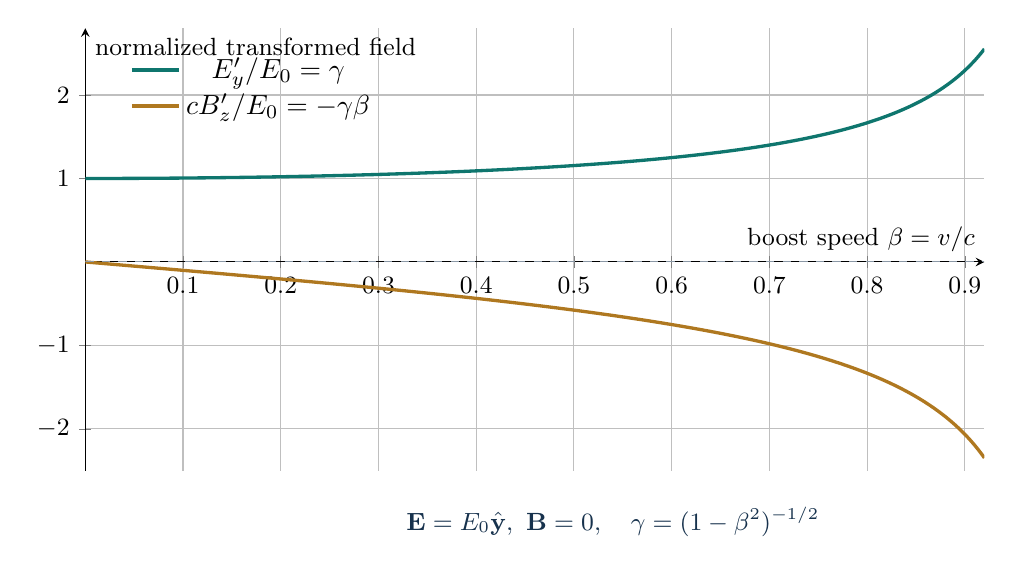
\begin{tikzpicture}
\begin{axis}[
 width=13cm,height=7.2cm,
 xmin=0,xmax=.92,ymin=-2.5,ymax=2.8,
 xlabel={boost speed $\beta=v/c$},ylabel={normalized transformed field},
 axis lines=middle,grid=both,
 legend style={draw=none,fill=none,at={(.04,.96)},anchor=north west},
 tick label style={font=\small},label style={font=\small},
]
 \addplot[accent,very thick,domain=0:.92,samples=301]
   {1/sqrt(1-x^2)};
 \addlegendentry{$E'_y/E_0=\gamma$}
 \addplot[gold!90!black,very thick,domain=0:.92,samples=301]
   {-x/sqrt(1-x^2)};
 \addlegendentry{$cB'_z/E_0=-\gamma\beta$}
 \addplot[ink!50,dashed,domain=0:.92]{0};
\end{axis}
\node[ink,font=\small] at (6.7,-.65)
 {$\mathbf E=E_0\hat{\mathbf y},\ \mathbf B=0,\quad
 \gamma=(1-\beta^2)^{-1/2}$};
\end{tikzpicture}
\end{document}
